

\tikzset{every picture/.style={line width=0.75pt}} %set default line width to 0.75pt        

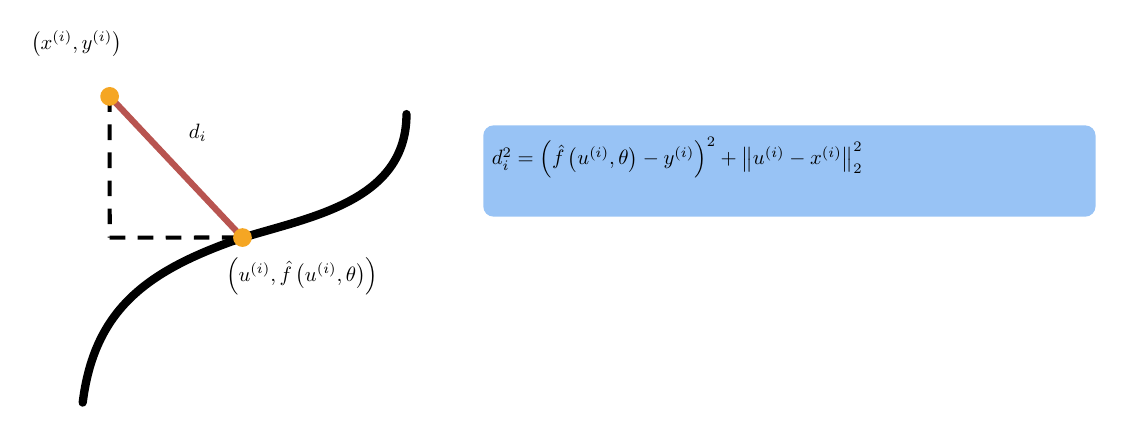
\begin{tikzpicture}[x=0.75pt,y=0.75pt,yscale=-1,xscale=1]
%uncomment if require: \path (0,300); %set diagram left start at 0, and has height of 300

%Shape: Free Drawing [id:dp5002881259079404] 
\draw  [color={rgb, 255:red, 0; green, 0; blue, 0 }  ][line width=3] [line join = round][line cap = round] (63.01,245.57) .. controls (68.41,202.42) and (91.96,183.67) .. (133.01,168.57) .. controls (164.12,157.14) and (219.01,152.23) .. (219.01,106.57) ;
%Straight Lines [id:da19530315633268636] 
\draw [color={rgb, 255:red, 184; green, 84; blue, 80 }  ,draw opacity=1 ][line width=2.25]    (75.99,98.05) -- (139.99,166.05) ;
%Straight Lines [id:da6781226747978477] 
\draw [line width=1.5]  [dash pattern={on 5.63pt off 4.5pt}]  (75.99,98.05) -- (76.01,166.1) ;
%Straight Lines [id:da3955370838358767] 
\draw [line width=1.5]  [dash pattern={on 5.63pt off 4.5pt}]  (76.01,166.1) -- (139.99,166.05) ;
%Shape: Circle [id:dp03457846112388152] 
\draw  [color={rgb, 255:red, 245; green, 166; blue, 35 }  ,draw opacity=1 ][fill={rgb, 255:red, 245; green, 166; blue, 35 }  ,fill opacity=1 ] (135.98,166.05) .. controls (135.98,163.84) and (137.77,162.04) .. (139.99,162.04) .. controls (142.2,162.04) and (144,163.84) .. (144,166.05) .. controls (144,168.27) and (142.2,170.06) .. (139.99,170.06) .. controls (137.77,170.06) and (135.98,168.27) .. (135.98,166.05) -- cycle ;
%Shape: Circle [id:dp15280043442217006] 
\draw  [color={rgb, 255:red, 245; green, 166; blue, 35 }  ,draw opacity=1 ][fill={rgb, 255:red, 245; green, 166; blue, 35 }  ,fill opacity=1 ] (71.98,98.05) .. controls (71.98,95.84) and (73.77,94.04) .. (75.99,94.04) .. controls (78.2,94.04) and (80,95.84) .. (80,98.05) .. controls (80,100.27) and (78.2,102.06) .. (75.99,102.06) .. controls (73.77,102.06) and (71.98,100.27) .. (71.98,98.05) -- cycle ;

% Text Node
\draw (37,65.44) node [anchor=north west][inner sep=0.75pt]  [xscale=0.75,yscale=0.75]  {$\left( x^{( i)} ,y^{( i)}\right)$};
% Text Node
\draw (113,110.4) node [anchor=north west][inner sep=0.75pt]  [xscale=0.75,yscale=0.75]  {$d_{i}$};
% Text Node
\draw  [color={rgb, 255:red, 0; green, 0; blue, 0 }  ,draw opacity=0 ][fill={rgb, 255:red, 152; green, 195; blue, 245 }  ,fill opacity=1 ]  (256,117) .. controls (256,114.24) and (258.24,112) .. (261,112) -- (546,112) .. controls (548.76,112) and (551,114.24) .. (551,117) -- (551,151) .. controls (551,153.76) and (548.76,156) .. (546,156) -- (261,156) .. controls (258.24,156) and (256,153.76) .. (256,151) -- cycle  ;
\draw (259,116.4) node [anchor=north west][inner sep=0.75pt]  [xscale=0.75,yscale=0.75]  {$d_{i}^{2} =\left(\hat{f}\left( u^{(i)} ,\theta \right) -y^{(i)}\right)^{2} +\left\Vert u^{(i)} -x^{(i)}\right\Vert _{2}^{2}$};
% Text Node
\draw (131,174.4) node [anchor=north west][inner sep=0.75pt]  [xscale=0.75,yscale=0.75]  {$\left( u^{(i)} ,\hat{f}\left( u^{(i)} ,\theta \right)\right)$};


\end{tikzpicture}